\section{Security}
\subsection{Pericoli della rete}
I protocolli di rete sono intrinsecamente non sicuri in quanto sono stati pensati in un periodo in cui la sicurezza non era qualcosa di importante.
Per questo motivo possono essere eseguiti alcuni attacchi ai vari protocolli.

\subsubsection{Packet sniffing}
Le trasmissioni su media in broadcast come ethernet o wireless sono soggetti a packet sniffing cioè un utente malevole è capace di catturare tutto il traffico in transito e carpire le informazioni comunicate tra i due endpoint della comunicazione.

\subsubsection{IP spoofing}
Non essendoci autenticazione sull' indirizzo IP un host può forgiare pacchetti con indirizzi IP sorgente diversi dal proprio e fingersi questo secondo host.

\subsubsection{Denial of Service}
Un folto gruppo di utenti organizzato può saturare di traffico un server e farlo collassare, in questo modo il server non può più fornire il suo servizio, è una negazione di servizio.
Di solito l' attacco è distribuito: Distributed Denial of Service ed il gruppo sorgente dell' attacco è detto \emph{botnet}.

\subsubsection{Replay attack}
Essendo il traffico in chiaro molto spesso possiamo pensare di catturare porzioni del traffico e re-inoltrarlo così com'è a piacere.

\subsubsection{Malware}
Si potrebbe usare la rete per iniettare codice malevolo all' interno degli hosts.
Tra questi malware possiamo annoverare gli spyware che si occupano di registrare la tastiera, i siti visitati e tante altre informazioni sull' utente.
Possiamo pensare di arruolare gli host in una botnet per portare avanti attacchi DDoS.

\subsection{Come proteggersi?}
La prima forma di protezione è la consapevolezza, eseguire programmi arbitrari scaricati dalla rete potrebbe essere dannoso ad esempio.

Gli aspetti di interesse per una comunicazione sono:
\begin{itemize}
    \item confidenzialità: solo il mittente ed il destinatario scelto dovrebbero poter comprendere il contenuto del messaggio.
    
    \item autenticazione: il mittente ed il destinatario vogliono essere certi di star parlando l' uno con l' altro e non con qualcuno che si spaccia come tale
    
    \item integrità: il mitente ed il destinatario vogliono essere sicuri che il messaggio non venga alterato durante la trasmissione
    
    \item accesso e disponibilità: il servizio proposto deve essere accessibile e disponibile
\end{itemize}
per alcuni scopi sono importanti solo alcune caratteristiche, per altri tutte quante.

\subsection{Crittografia}
Per ottenere tutte o alcune di queste proprietà possiamo usare la crittografia!
Più genericamente possibile la crittografia si occupa di prendere un messaggio \emph{in chiaro} e di restituirne un altro in forma cifrata utilizzando un algoritmo di cifratura ed una chiave.
Per gli utilizzi comuni l' algoritmo è noto a tutti e pubblico mentre le chiave (o le chiavi) sono note solo agli endpoint della comunicazione.
Diremo:
\begin{itemize}
    \item $m$ testo in chiaro
    \item $K_A(m)$ testo cifrato con algoritmo $K$ e chiave $A$
    \item $m = K_B(K_A(m))$ applicando l' algoritmo di decifrazione con la chiave di decifratura sul messaggio cifrato si riottiene il messaggio in chiaro
\end{itemize}

Possiamo discernere gli algoritmi crittografici in varie classi in base allo schema che si utilizza.

\subsubsection{Crittografia simmetrica}
La chiave di cifratura e la chiave di decifratura sono identiche, è un segreto condiviso.
Prima di potersi scambiare dei messccaaggi occorre quindi mettersi d' accordo sulla chiave comune da utilizzare.

\subsubsection{Cifrario di Cesare}
Un esempio di cifrario simmetrico è il cifrario di Cesare, si tratta di un cifrario a sostituzione che sostituisce ad ogni lettera la lettera che lo segue ad una distanza $k$.
Possiamo pertanto costruire una tabella di corrispondenza che sostituisce ad ogni lettera un' altra e per cifrare non ci basta che scorrere questa tabella di corrispondenza mentre per decriptare si scorre la tabella nel senso contrario.

La chiave in questo schema crittografico è il numero di shift da eseguire.

\subsubsection{Sostituzione monoalfabetica}
E' la versione generale del cifrario di Cesare che associa una sostituzione arbitraria.
In questo caso la chiave è la tabella che associa l' alfabeto originale alla sua versione cifrata.

\subsubsection{Sostituzione polialfabetica}
In questo metodo anziché cifrare una lettera sempre con la stessa si scelgono varie tabelle di sostituzione monoalfabetica e si usano tutte seguendo un determinato pattern.
Con questo algoritmo lo spazio delle chiavi è estremamente elevato e difficilmente attaccabile tramite altri metodi.

\subsubsection{Crittografia simmetrica moderna}
La crittografia simmetrica moderna si divide in due macro categorie:
\begin{itemize}
    \item cifrari a flusso: cifra un bit per volta
    \item cifrario a blocco: cifra singoli blocchi di plaintext e cifra ognuno di essi singolarmente
\end{itemize}

Per misurare la sicurezza di un algoritmo di misura il tempo ipoteticamente necessario a romperlo con qualsiasi metodo.

\subsubsection{DES - Data Encryption Standard}
E' uno dei primi cifrari a blocchi che prevede chiavi di 56 bit, il DES è poco sicuro e pertanto poco utilizzato odiernamente in quanto si rompe facilmente tramite una ricerca esaustiva ed altri tipi di attacchi.

Una versione più sicura costruita sulla base del DES è il triplo DES che usa tre chiavi differenti ed esegue in sequenza: encryption, decryption ed encryption.
Anche questa versione tuttavia soffre di alcune lacune.

\subsubsection{AES - Advanced Encryption Standard}
L' algoritmo crittografico più usato oggi è l' AES che prevede chiavi a 128, 192 o 256 bit.

\subsubsection{Scambio delle chiavi}
La crittografia simmetrica ha un grande problema: lo scambio delle chiavi.
Essendo uguale per entrambi gli endpoint la chiave non può essere inviata in chiaro sul canale di comunicazione perché potrebbe venire carpita e quindi utilizzata per decriptare anche dagli estranei.

Un metodo sarebbe quello dello scambio diretto in persona ma non sempre i due endpoint possono incontrarsi per scambiarsi la chiave di persona.

Possiamo usare come rifermento un centro di distribuzione delle chiavi ma dovrebbe essere una entità certificata ed affidabile per entrambi i partecipanti.

Possiamo utilizzare la crittografia a chiave pubblica, che è il metodo moderno.

\subsubsection{Crittografia a chiave pubblica}
In questo schema crittografico ogni utente ha una coppia di chiavi:
\begin{itemize}
    \item chiave privata: conosciuta solo al possessore
    \item chiave pubblica: generata a partira dalla chiave privata e resa pubblica per tutti
\end{itemize}

Per inviare un messaggio si prende il plaintext e lo si cifra con la chiave pubblica del destinatario, per decifrare è necessario ricorrere alla chiave privata del destinatario, essendo privata e nota solo a lui si ha la confidenzialità delle informazioni, inoltre non dobbiamo effettuare uno scambio delle chiavi in quanto quella pubblica è nota a tutti.

\subsubsection{RSA}
L' algoritmo di crittografia asimmetrica più conosciuto è quello RSA (Rivest, Shamir, Adleman) che gode di una importante proprietà: applicare prima la chiave pubblica e poi quella privata è equivalente ad applicare prima quella privata e poi quella pubblica.

\subsubsection{Chiavi di sessione}
Dal momento che gli algoritmi asimmetrici sono molto meno efficienti in termini computazionali li usiamo per scambiare una chiave e successivamente la vera e propria comunicazione avviene mediante crittografia simmetrica.
La chiave che ci si scambia è unica per ogni sessione di comunicazione, quindi la chiave prende il nome di \emph{chiave di sessione}.

\subsection{Integrità ed autenticazione}
Permette ai partecipanti della comunicazione di verificare che il messaggio ricevuto è autentico.
Inoltre l' integrità garantisce:
\begin{itemize}
    \item che la sorgente sia chi penso che sia
    \item che il contenuto del messaggio non venga alterato
    \item che il messaggio non possa essere replicato
    \item che la sequenza dei messaggi sia mantenuta correttamente
\end{itemize}

\subsubsection{Message Digest}
Un digest di un messaggio è il risultato di una funzione hash con ingresso il messaggio stesso.
Chiamiamo il digest $H(m)$.

Alcune proprietà importanti di queste funzione sono:
\begin{itemize}
    \item facile da calcolare
    \item difficile da invertire (irreversibile)
    \item deve restituire un messaggio di lunghezza fissa partendo da messaggi di lunghezza arbitraria
    \item resistente alle collisioni, cioè deve essere difficile trovare due input che ci danno lo stesso output
    \item deve produrre un output che sembri randomico
\end{itemize}

\subsubsection{Message Authentication Code - MAC}
Preso un messaggio ed un segreto condiviso eseguiamo l' hash della concatenazione dei due, questo valore lo inviamo assieme al messaggio stesso.
Chi riceve il messaggio per accertarsi che sia autenticato deve solamente eseguire nuovamente l' algoritmo di hashing sul messaggio ed il segreto condiviso, se è identico al MAC ricevuto allora il messaggio non è stato modificato.

\begin{figure}[H]
    \centering
    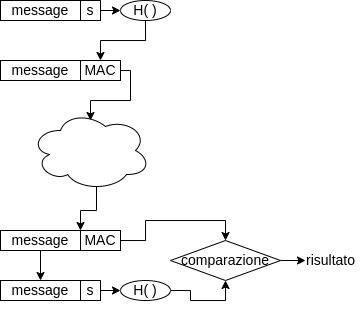
\includegraphics[width=300px]{images/7_Security/Message_authentication_code.png}
\end{figure}

Questo metodo funziona se il segreto è conosciuto solo ed esclusivamente dai due endpoint della comunicazione.

Oltre a provare l' integrità del messaggio il MAC funge anche da autenticazione in quanto il segreto è noto solo alle due controparti.

L' algoritmo HMAC è una versione di MAC standardizzata che usa gli algoritmi di hash MD5 e SHA-1:
\begin{itemize}
    \item concatenare segreto e messaggio
    \item hashare la concatenazione
    \item concatenare l' hash ottenuto al messaggio
    \item hashare la nuova concatenazione
\end{itemize}

\subsubsection{Esempio con OSPF - Open Shortest Path First}
OSPF è un algoritmo di routing quindi permette l' advertising delle route.
Si potrebbe quindi pensare di fingersi un router ed inviare pacchetti forgiati a piacere, oppure cancellare pacchetti in modo che non arrivino a destinazione o addirittura modificarli.
Ci serve un meccanismo di autenticazione dei messaggi, OSPF mette a disposizione 3 metodi:
\begin{itemize}
    \item nessuna autenticazione
    \item password condivisa tra tutti i nodi che però viene inserita in chiaro in un campo del pacchetto OSPF
    \item autenticazione con hash crittografico: si fa un hash del pacchetto OSPF e della chiave segreta condivisa, quindi si concatena al pacchetto OSPF
\end{itemize}

\subsubsection{Firma digitale}
E' un meccanismo crittografico analogo alla firma cartacea:
\begin{itemize}
    \item verificabile: chi riceve il messaggio può verificare che il mittente sia chi effettivamente dice di essere
    
    \item non forgiabile: il mittente può e solo lui può effettuare la firma
    
    \item non ripudiabilità: il ricevente può provare che il mittente ha firmato un messaggio e non un altro
    
    \item integrità del messaggio: il mittente può provare che ha firmato un messaggio e non un altro
\end{itemize}
Il MAC non può essere utilizzato come firma digitale in quanto il segreto è conosciuto da almeno due enti quindi ognuno dei due potrebbe firmare a nome dell' altro, vengono meno la verificabilità, la non forgiabilità e la non ripudiabilità.

La firma digitale deve quindi essere creata usando la crittografia a chiave pubblica: il mittente cifra il messaggio con la sua chiave privata e gli altri usano la sua chiave pubblica per decifrarlo.
Se la chiave privata è effettivamente privata allora solo un utente può forgiare i messaggi, quindi è verificabile.

Abbiamo tuttavia detto che cifrare con la crittografia a chiave pubblica è dispendioso e non si può fare per messaggi troppo lunghi, la soluzione è quindi firmare un hash del messaggio e non il messaggio stesso:
\begin{itemize}
    \item Il mittente invia la concatenazione del messaggio con la firma dell' hash del messaggio
    
    \item Il destinatario per autenticare il messaggio deve eseguire l' hash del messaggio e confrontare che sia uguale all' hash decifrato con la chiave pubblica
\end{itemize}

\begin{figure}[H]
    \centering
    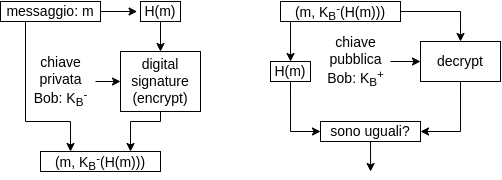
\includegraphics[width=330px]{images/7_Security/signed_MAC.png}
\end{figure}

Tutta questa teoria si basa sull' assunto che la chiave pubblica che si utilizza per verificare sia effettivamente la chiave pubblica associata alla chiave privata usata per firmare, questo assunto non sempre è vero, l' attaccante potrebbe ad esempio aver intercettato e sostituito la chiave pubblica durante la trasmissione tra i due che comunicano.

\subsubsection{Certification of authority}
E' un ente che collega le chiavi pubbliche agli utenti attraverso un certificato.
Chi depone la propria chiave pubblica deve fornire documentazione in modo che la CA si accerti dell' identità, la CA crea il certificato inserendo all' interno le informazioni circa l' utente e lo firma con la propria chiave privata.

Quando un utente vuole la chiave pubblica di un altro utente la chiede alla CA, gli viene fornito un certificato che può controllare tramite la chiave pubblica della CA.
Ogni CA a sua volta è certificata da un' altra authority in uno schema ad albero alla radice del quale c'è un organo ritenuto affidabile.

\subsubsection{Certificato}
E' un documento digitale che contiene la chiave pubblica assieme alle informazioni del proprietario della chiave pubblica.
Viene inoltre firmato dall' autorità che lo rilascia.

Ha un formato standardizzato in RFC 2459.

\subsubsection{Attacchi playback}
Supponiamo di eseguire un pagamento e di chiedere alla nostra banca di effettuarlo, seppure il messaggio è criptato possiamo registrarlo e reinviarlo a piacere per ri-eseguire questa transazione.

Per risolvere questo problema nel messaggio di transazione si embedda un valore casuale che cambia ad ogni messaggio, la stessa banca ci dice di utilizzare questo determinato valore quindi se andiamo ad eseguire altre richieste, essendo cambiato questo valore, non possiamo utilizzare messaggi pre-registrati.

\begin{figure}[H]
    \centering
    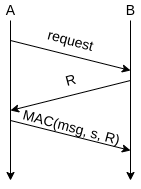
\includegraphics[width=100px]{images/7_Security/nonce_usage.png}
\end{figure}

\subsection{Mettere in sicurezza le email}
Per mettere in sicurezza le email dovrei ottenere:
\begin{itemize}
    \item confidenzialità
    \item autenticazione del mittente
    \item autenticazione del destinatario
    \item integrità del messaggio
\end{itemize}

Un primo schema che garantisca confidenzialità ed integrità prevede la cifratura del messaggio con un algoritmo simmetrico, la chiave utilizzata invece la si cifra con la chiave pubblica del destinatario.
Il destinatario non deve fare altro che decriptare la chiave simmetrica utilizzando la propria chiave privata e decriptare il messaggio cifrato con la chiave segreta ottenuta.

Per ottenere l' autenticazione nello schema possiamo aggiungere al messaggio un hash del messaggio firmato con la chiave privata del mittente, il destinatario deve quindi eseguire l' hash del messaggio ricevuto e confrontarlo con il risultato della decifratura dell' hash ricevuto.

\subsubsection{PGP - Pretty Good Privacy}
E' una suite software che prevede algoritmi simmetrici ed asimmetrici, funzioni hash ed algoritmi di firma digitale.
E' lo standard de-facto per lo scambio di email in sicurezza.
NB: il creatore Phil Zimmerman è stato indagato per 3 anni dopo aver reso pubblico questo software.

\subsection{SSL (Secure Socket Layer) e TCP/IP}
SSL è un protocollo che viene posizionato tra il livello di trasporto ed il livello di applicazione, si tratta di un middleware quindi.
Mette a disposizione del programmatore delle API per fornire crittografia a livello applicazione senza preoccuparsi della implementazione ma pensando solo alla logica dell' applicazione.

Permette di ottenere confidenzialità, integrità dei dati ed autenticazione degli endpoint, gli obiettivi principali per i quali è stato creato sono la messa in sicurezza delle transazioni negli e-commerce, cifratura dei dati ed autenticazione del web server.
Si può anche utilizzare per autenticare i client ma spesso non si fa.

La versione più aggiornata è nota come TLS ed è descritta in RFC 2246.
Per utilizzarla si deve scrivere le proprie applicazioni utilizzando i secure socket anziché quelli normali.

Una versione semplificata di SSL lavora tramite:
\begin{itemize}
    \item Handshake
    \item Key derivation
    \item Data transfer
    \item Connection Closure
\end{itemize}

\subsubsection{Handshake}
I due endpoint usano i propri certificati e le proprie chiavi private per autenticarsi a vicenda e scambiarsi un segreto condiviso:
\begin{figure}[H]
    \centering
    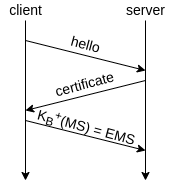
\includegraphics[width=100px]{images/7_Security/ssl_handshake.png}
\end{figure}

\subsubsection{Key derivation}
I due endpoint usano lo shared secret per derivare un insieme di chiavi di sessione:
\begin{itemize}
    \item $K_c$ chiave per criptare i dati dal client verso il server
    \item $M_c$ chiave per generare il MAC dal client al server
    \item $K_s$ chiave per criptare dati dal server al client
    \item $M_s$ chiave per generare il MAC dal server al client
\end{itemize}
le chiavi vengono prodotte utilizzando un algoritmo di derivazione delle chiavi.

\subsubsection{Data Transfer}
I dati da trasferire sono suddivisi in una serie di blocchi detti \emph{record}, ogni blocco ha un MAC posizionato alla fine del record.
Per permettere record di diversa lunghezza e comunque poter discernere tra dati e MAC si inserisce un campo lunghezza all' inizio.

Per impedire attacchi di record \& playback si inserisce nei record un numero di sequenza usato per computare il MAC, in questo modo anche replicando il record il MAC computato sarà diverso e quindi il record verrà droppato.

Per evitare truncation attacks, cioè una terminazione improvvisa della connessione, si usa un campo di \emph{tipo}, anch' esso usato nel calcolo del MAC.

\subsubsection{Record SSL}
La struttura di un record è:
\begin{figure}[H]
    \centering
    
\includegraphics[width=200px]{images/7_Security/ssl_record.png}
\end{figure}
$$ MAC = MAC(M_x, sequence||type||data) $$

\subsubsection{Connection closure}
Si usano messaggi speciali per chiudere la connessione per evitare alcuni problemi che potrebbero venire a crearsi.

\subsubsection{SSL completo}
Al protocollo che abbiamo pensato mancano alcune cose come la negoziazione della cipher suite: i due endpoint devono mettersi d' accordo su quali algoritmi utilizzare quindi devono scambiarsi l' elenco degli algoritmi che effettivamente conoscono.
Una cipher suite deve contenere:
\begin{itemize}
    \item un algoritmo a chiave pubblica
    \item un algoritmo simmetrico
    \item un algoritmo per il calcolo del MAC
\end{itemize}

Nel protocollo SSL completo durante l' handshake si deve quindi:
\begin{itemize}
    \item autenticare il server
    \item negoziare una cipher suite che sia implementata in entrambi gli endpoint della comunicazione
    \item stabilire delle chiavi
    \item autenticare il client (non obbligatoriamente)
\end{itemize}

La negoziazione della cipher suite avviene come segue:
\begin{enumerate}
    \item il client invia al server la lista completa degli algoritmi che può supportare, insieme ad un nonce

    \item il server sceglie da questa lista di algoritmi e li comunica al client assieme al proprio certificato ed un secondo nonce
    
    \item il client verifica il certificato, ne estrae la chiave pubblica, genera un pre-master-secret e lo cifra con la chiave pubblica del server, glielo comunica
    
    \item client e server costruiscono indipendentemente le chiavi a partire dal pre-master-secret
    
    \item il client invia il MAC di tutto l' handshake
    
    \item il server invia il MAC di tutto l' handshake
\end{enumerate}
Gli utlimi due passaggi prevengono l' handshake dal tampering in quanto un attacco man-in-the-middle potrebbe modificare la lista degli algoritmi del client eliminando gli algoritmi forti e lasciando solo quelli deboli.

I nonce inviati dal client e dal server sono utilizzati per evitare attacchi reply in quanto: se io prendo tutti i messaggi del client e provo a reinviarli fingendomi lui, il server mi risponderà con un nonce diverso da quello della prima volta quindi le chiavi crittografiche cambieranno e l' attacco non potrà essere portato avanti.

\subsection{VPN e IPsec}
Le Virtual Private Network permettono di creare delle reti completamente separate dall' internet pubblica sfruttando l' internet pubblico stesso.
Creare una rete separata da internet sarebbe molto dispendioso perché richiederebbe una intera infrastruttura di rete a parte, invece possiamo sfruttare la rete che già esiste: il traffico interno ad una rete aziendale lo spediamo attraverso la Internet pubblica ma lo inviamo criptato.

Una implementazione delle VPN si ottiene utilizzando il protocollo IPsec, implementato sui router o sui singoli host che si occupa di prendere i datagrammi IP, rimpiazzare il payload con un header IPsec ed il payload criptato.
Ovviamente alla ricezione bisogna prendere l' header IPsec ed il payload criptato e svolgere le azioni al contrario.

Questo protocollo permette l' integrità dei dati, autenticazione della sorgente, previene gli attacchi di tipo replay e provvede alla confidenzialità dei dati.
Questo servizio può essere fornito attraverso due protocolli:
\begin{itemize}
    \item Authentication header (AH): fornisce l' autenticazione della sorgente e l' integrità dei dati, ma non la confidenzialità
    \item Encapsulation Security Protocol (ESP): fornisce autenticazione della sorgente, integrità dei dati e confidenzialità
\end{itemize}
Parleremo di ESP.

Qualsiasi VPN prevede, prima di inviare qualsiasi dato, la creazione di una connessione virtuale tra le due entità della comunicazione, questa connessione viene chiamata \emph{Security Association}, queste sono simplex quindi permettono ad un host di parlare e ad un altro di ascoltare, quindi se ci sono $N$ nodi che vogliono partecipare alla rete ci vogliono $2 + 2N$ security association (contando anche quelle del quartier generale).

Entrambi i nodi della comunicazione mantengono informazioni sugli stati della connessione (quindi rendono IP un protocollo connection-oriented):
\begin{itemize}
    \item security parameter index: stringa da 32 bit che individua la SA che l' host sta gestendo
    \item IP della interfaccia di origine
    \item IP della interfaccia di destinazione
    \item tipo di cifratura utilizzato
    \item chiave di cifratura
    \item tipo del controllo di integrità (HMAC, ecc)
    \item chiave di autenticazione (segreto per il MAC)
\end{itemize}
Tutte queste informazioni sono all' interno del Security Association Database (SAD).

Un datagramma IPsec che utilizza il protocollo ESP è costituito:
\begin{figure}[H]
    \centering
    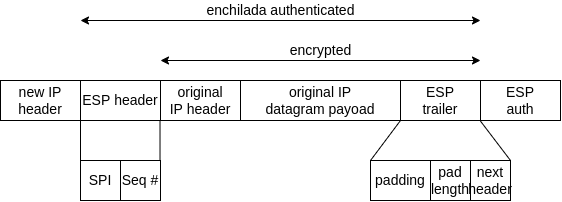
\includegraphics[width=330px]{images/7_Security/IPsec_datagram.png}
\end{figure}
NB: il padding nel trailer serve per rendere il contenuto un multiplo intero del blocco affinché si possano usare gli algoritmi di crittografia a blocchi.

Così facendo abbiamo eseguito una encapsulation del vecchio datagramma IP in uno nuovo ma con il payload criptato.

Come fa un router a sapere quali datagrammi deve incapsulare e quali no?
All' interno del router si trova un Security Policy Database (SPD) che dato un datagramma ne controlla IP sorgente e destinatario ed il numero di protocollo ed in base a questi dati cerca nella sua tabella interna se usare IPsec ed in tal caso quale security association utilizzare.

\subsection{Firewalls}
E' un dispositivo hardware o software che si utilizza per isolare la rete interna dall' Internet permettendo solo ad alcuni pacchetti di entrare e/o uscire bloccando tutti gli altri.

\subsubsection{Perché?}
Permette di mitigare attacchi di tipo DoS perché ci permette di isolare quegli host che generano tanto traffico o richieste SYN che poi non vengono concluse.
Previene modifiche ed accessi illeciti a dati interni alla rete.
Permette l' accesso alla rete solo ad elementi autorizzati.

\subsubsection{Tipologie}
Riconosciamo tre tipologie di firewall:
\begin{itemize}
    \item stateless packet filters
    \item stateful packet filters
    \item application gateways
\end{itemize}

\subsubsection{Stateless packet filtering}
Il router applica dei filtri sui singoli pacchetti decidendo se fare forward o dropparli in base a:
\begin{itemize}
    \item IP sorgente e destinazione
    \item porta sorgente e destinazione
    \item messaggi ICMP
    \item i flag dei pacchetti TCP
\end{itemize}

Queste regole vengono indicate compilando delle apposite \emph{Access Control List} che indicano l' azione da intraprendere sul filtro selezionato.
Le regole si leggono dall' alto verso il basso, la prima che matcha il pacchetto che si sta elaborando viene eseguita.
Alla fine si inserisce una \emph{deny all} oppure una \emph{allow all}, ovviamente si consiglia di utilizzare una deny all in quanto è una opzione più sicura.

Esempio di ACL:
\begin{table}[ht!]
    \centering
    \begin{tabular}{c|c|c|c|c|c|c}
        action & \thead{source \\ address} & \thead{dest \\ address} & protocol & \thead{source \\ port} & \thead{dest \\ port} & \thead{flag \\ bit}  \\
        \hline
        allow & 222.22/16 & \thead{outside of \\ 222.22/16} & TCP & $>$1023 & 80 & any \\ 
        allow & \thead{outside of \\ 222.22/16} & 222.22/16 & TCP & 80 & $>$1023 & ACK \\
        allow & 222.22/16 & \thead{outside of \\ 222.22/16} & UDP & $>$1023 & 53 & --- \\
        allow & \thead{outside of \\ 222.22/16} & 222.22/16 & UDP & 53 & $>$1023 & --- \\ 
        deny & all & all & all & all & all & all \\ 
    \end{tabular}
\end{table}

\subsubsection{Stateful packet filtering}
Permette il filtering dei pacchetti con coscienza del loro stato all' interno della comunicazione.
Traccia l' inizio e la fine della connessione TCP in modo da sapere se i pacchetti in transito hanno senso, inoltre applica dei timeout alle connessioni in modo da droppare i pacchetti di connessioni scadute.

Anche in questo caso si utilizzano delle ACL con però le opzioni per tracciare lo stato come ad esempio i bit flaggati.

Esempio di ACL:
\begin{table}[ht!]
    \centering
    \begin{tabular}{c|c|c|c|c|c|c|c}
        action & \thead{source \\ address} & \thead{dest \\ address} & proto & \thead{source \\ port} & \thead{dest \\ port} & \thead{flag \\ bit} & \thead{check \\ conxion} \\
        \hline
        allow & 222.22/16 & \thead{outside of \\ 222.22/16} & TCP & $>$1023 & 80 & any & \\
        allow & \thead{outside of \\ 222.22/16} & 222.22/16 & TCP & 80 & $>$1023 & ACK & $\times$ \\
        allow & 222.22/16 & \thead{outside of \\ 222.22/16} & UDP & $>$1023 & 53 & --- & \\
        allow & \thead{outside of \\ 222.22/16} & 222.22/16 & UDP & 53 & $>$1023 & --- & $\times$ \\ 
        deny & all & all & all & all & all & all & \\ 
    \end{tabular}
\end{table}

\subsubsection{Application gateways}
Permette di applicare filtri ai dati così come ai campi IP e TCP/UDP, per esempio possiamo permette ad un utente interno alla rete di collegarsi in telnet all' esterno.
Si tratta di una macchina specifica adibita a ricevere determinato traffico e si occupa di spedirlo all' esterno, internamente ad una rete solo lui ha il permesso di inviare questo traffico quindi fa da middleware per tutti gli altri host.

Un esempio è un web proxy usato per filtrare in base ai domini o alle categorie.

\subsubsection{Limitazioni di firewall ed application gateway}
Se volessimo usare tante applicazioni che necessitano di un trattamento specifico dovremmo configurare un application gateway per ognuno di loro, questo comporta che il client che vuole usare quel software debba esserne a conoscenza e debba essere configurato per utilizzarlo.

Inoltre non eliminano tutte le possibili minacce: un utente malintenzionato interno alla rete o esterno ad essa potrebbe modificare l' IP sorgente di alcuni pacchetti eseguendo il così detto IP spoofing, in tal caso il router e gli eventuali firewall ed application gateway non possono essere certi della provenienza dei pacchetti.

\subsubsection{Intrusion Detection Systems}
Il normale packet filtering lavora esclusivamente sugli header TCP ed IP non eseguendo alcuna correlazione tra le varie sessioni.
Gli IDS invece possono eseguire una deep packet inspection, possono cioè guardare il contenuto dei pacchetti, ed anche esaminare correlazioni tra più pacchetti.
Sono capaci di accorgersi di eventuali port scanning, network mapping ed attacchi DoS.

Solitamente se ne inseriscono diversi nella rete in modo da segmentare la rete applicando diversi controlli sul traffico.
